\section{Descrizione procedura di Autoranging presente nel Firmware}

\begin{frame}{Modalità di Autoranging inclusa nel Firmware}  
  \begin{center}
    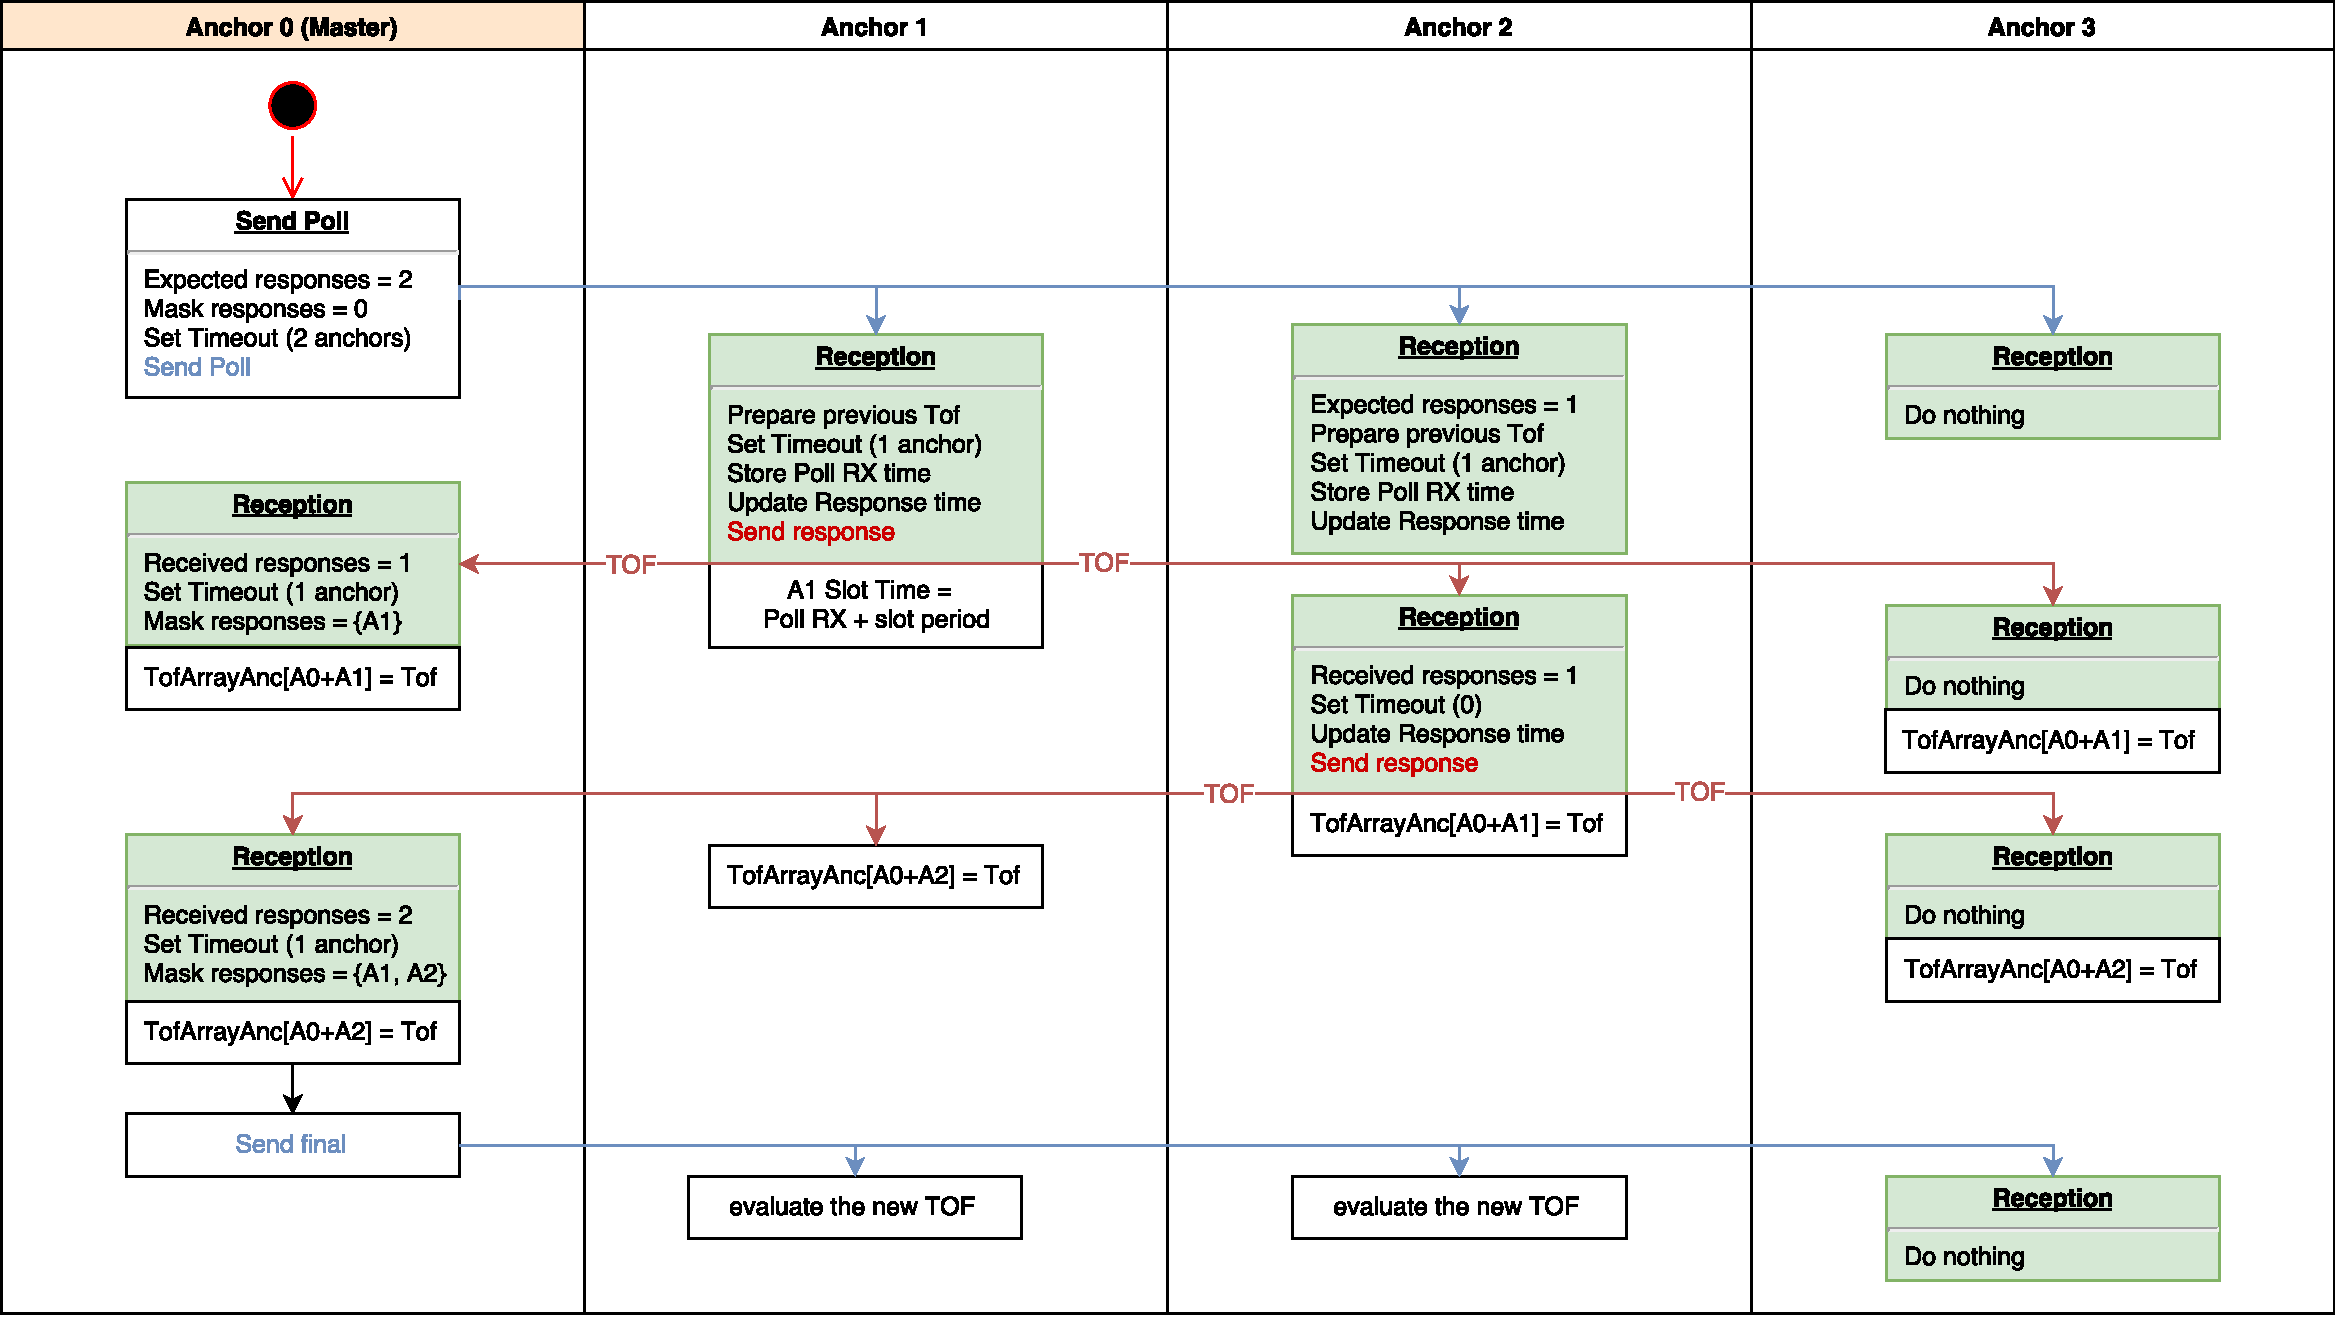
\includegraphics[width=\linewidth]{A2A_oldA0.pdf}
  \end{center}
\end{frame}

\begin{frame}{Modalità di Autoranging inclusa nel Firmware}
  \begin{center}
    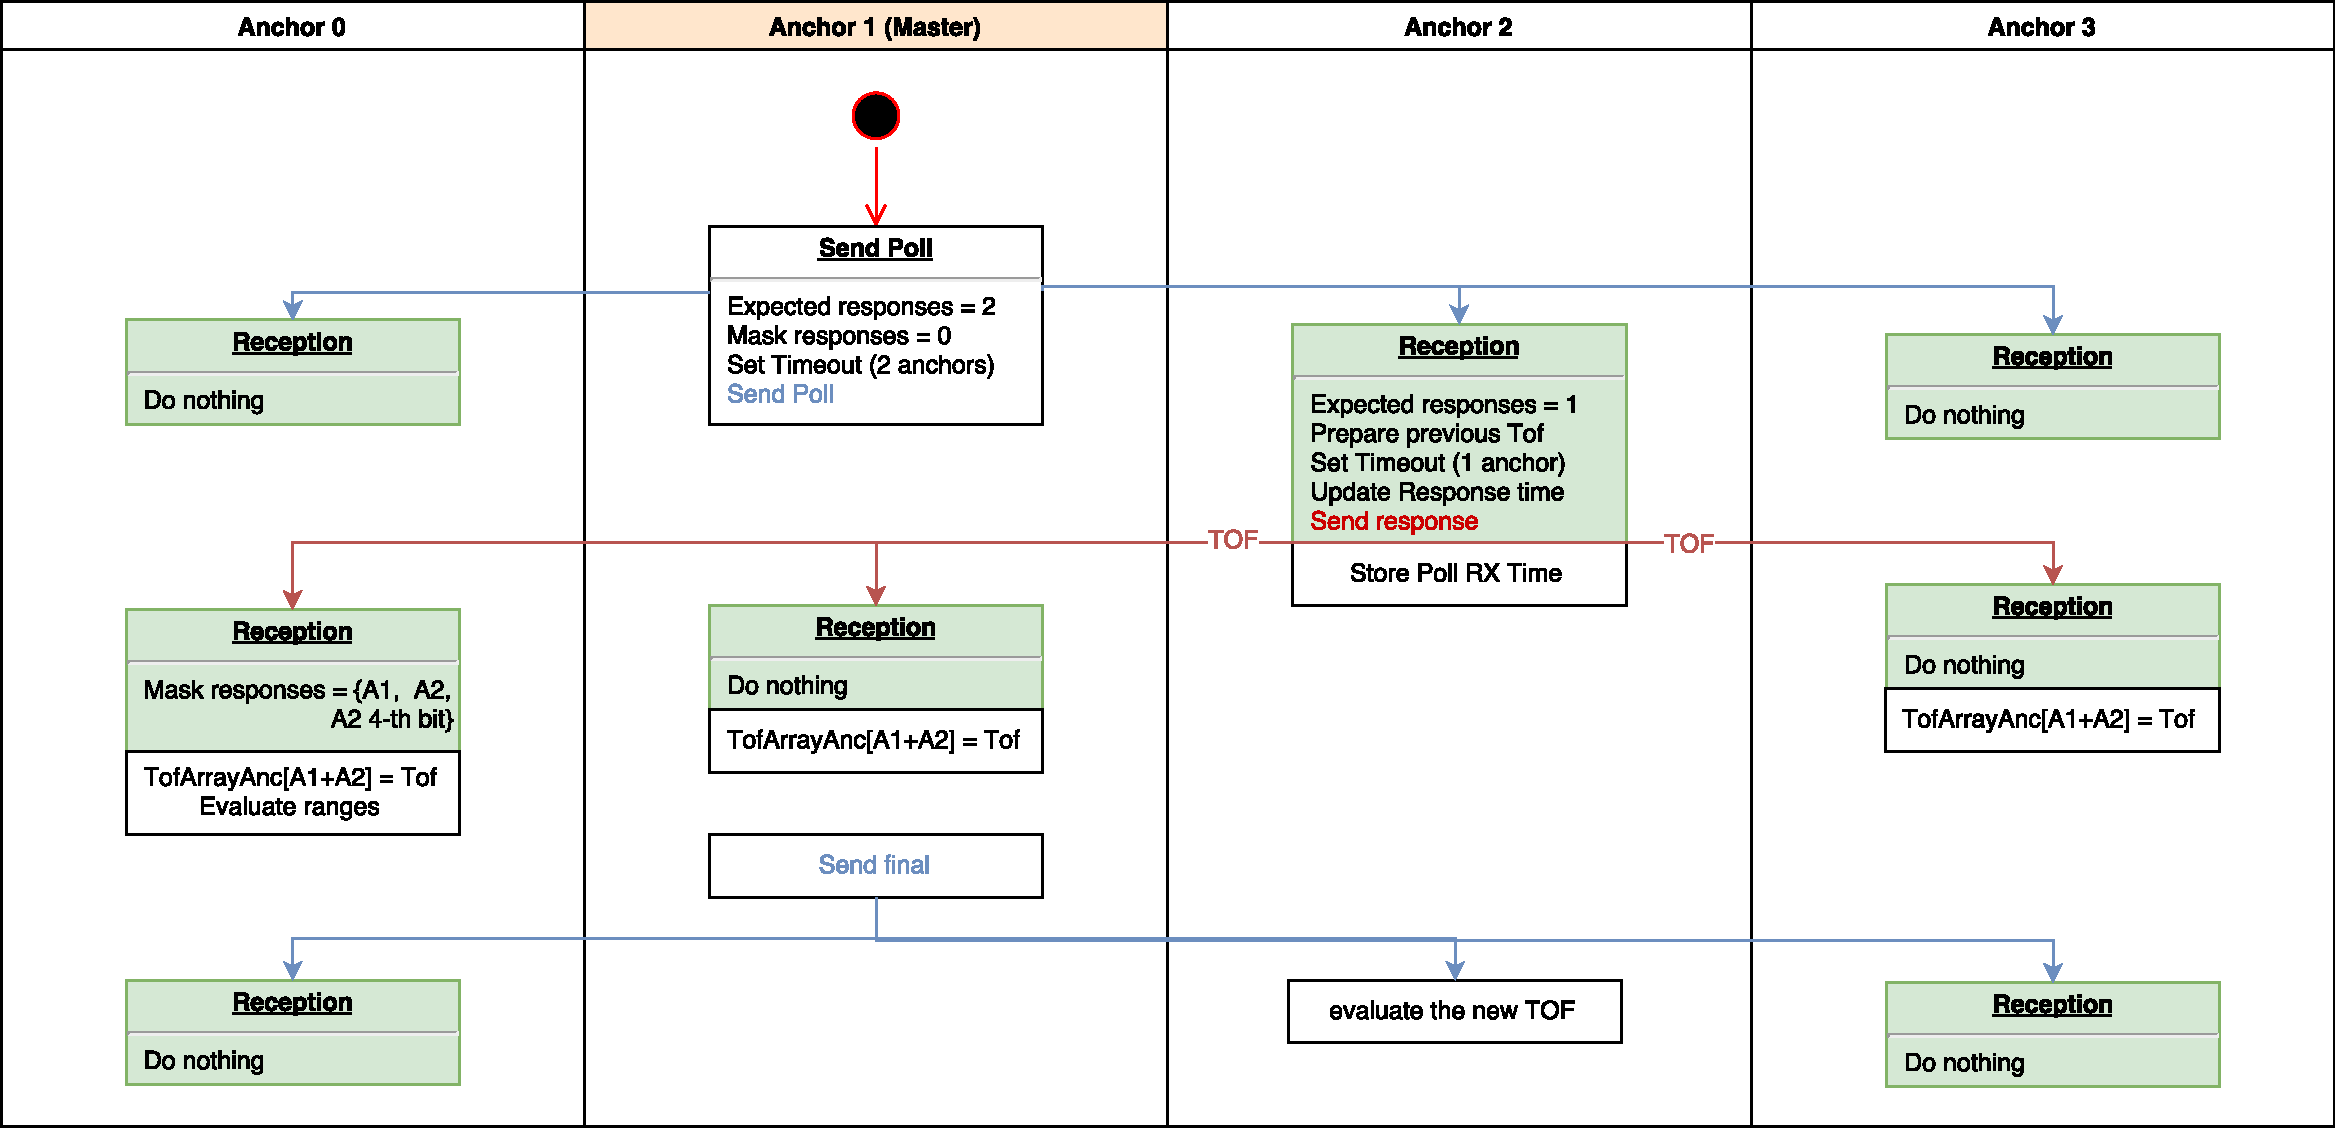
\includegraphics[width=\linewidth]{A2A_oldA1.pdf}
  \end{center}
\end{frame}

\begin{frame}{Considerazioni}
  La procedura di autoranging presente nel firmware:
  \begin{itemize}
  \item [-] calcola solo 3 su 6 dei range richiesti per valutare la posizione delle ancore;
  \item [-] non spedisce i range calcolati / la loro media al tag;
  \item [-] è implementata mediante parti di codice specifiche per ogni ancora quindi \alert{non}
    facilmente estensibile al caso di più ancore;
  \item [-] a parita di scelta del superframe period e dello slot period \alert{riduce} di $N$ il numero
    massimo di tag utilizzabili poiché la procedura avviene negli ultimi $N$\footnote{nel caso del
      firmware $N = 2$} slot.
  \end{itemize}
\end{frame}

\section{Nuova procedura di autoranging}

\begin{frame}{Nuova procedura di autoranging}
  A differenza della procedura originale la nuova procedura \alert{non} avviene durante la fase
  di ranging portata avanti dal tag ma avviene in una fase preliminare durante la quale il tag sta in
  attesa.
  \par
  L'intera procedura si divide in 3 parti. Ogni ancora \alert{a turno}: 
  \begin{itemize}
  \item [1.] valuta $M$ volte i range di interesse, i.e. l'ancora
    j-esima raccoglie i range $r_{j,j+1}$ ... $r_{j,N-1}$ con $N$ il numero di ancore e $j<N$;
  \item [2.] calcola la media dei range raccolti;
  \item [3.] invia i range medi al tag ogni volta che risponde ad un suo Poll.
  \end{itemize}
\end{frame}

\begin{frame}{Simmetria}
  In linea di principio quando l'ancora j-esima esegua la sua fase di raccolta dei range non sarebbe
  necessario che le ancore con indice $i < j$ partecipino alla procedura poiché sono di interesse solo
  i range $r_{j,k}$ con $j < k < N$. Tuttavia facendo partecipare sempre tutte le ancore è possibile
  raccogliere per $M$ volte ciascun range eseguendo $M/2$ istanze di range per ogni ancora invece che $M$.

  \begin{exampleblock}{Numero di istanze di range richieste}
    Date $N$ ancore per raccogliere $M$ volte ciascun range di interesse sono richieste
    \[
    N \frac{M}{2}
    \]
    istanze di ranging
  \end{exampleblock}
\end{frame}

\begin{frame}{Simmetria - esempio}
  Sia $i<j$, l'ancora $A_i$ esegue $M/2$ istanze di ranging
  \begin{center}
    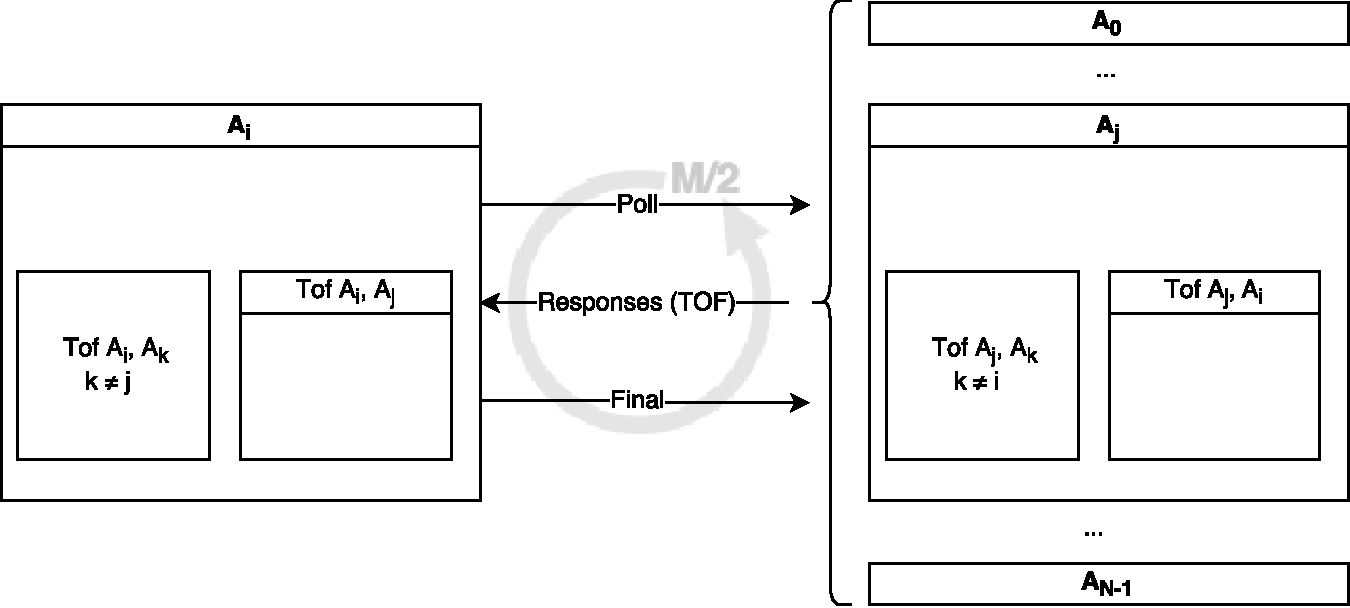
\includegraphics[width=\linewidth]{new_autoranging_1.pdf}
  \end{center}
\end{frame}

\begin{frame}{Simmetria - esempio}
  L'ancora $A_i$ ha memorizzato $M/2$ misure di ranging
  \begin{center}
    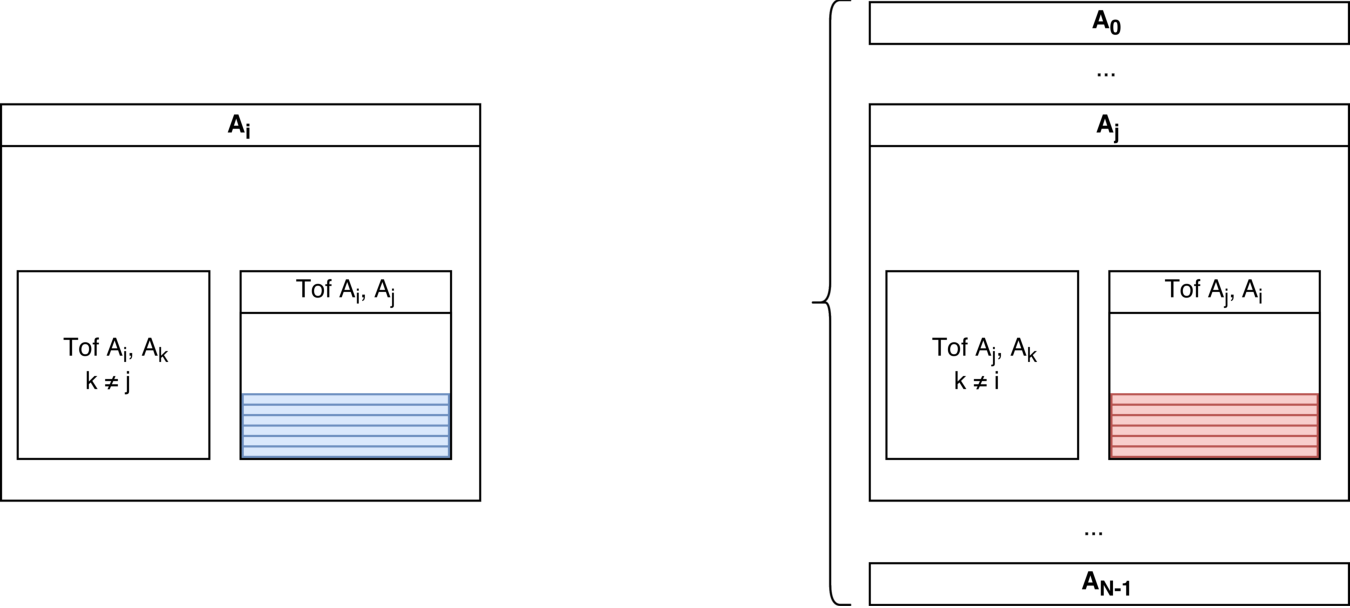
\includegraphics[width=\linewidth]{new_autoranging_2.pdf}
  \end{center}
\end{frame}

\begin{frame}{Simmetria - esempio}
  Successivamente l'ancora $A_j$ esegue $M/2$ istanze di ranging
  \begin{center}
    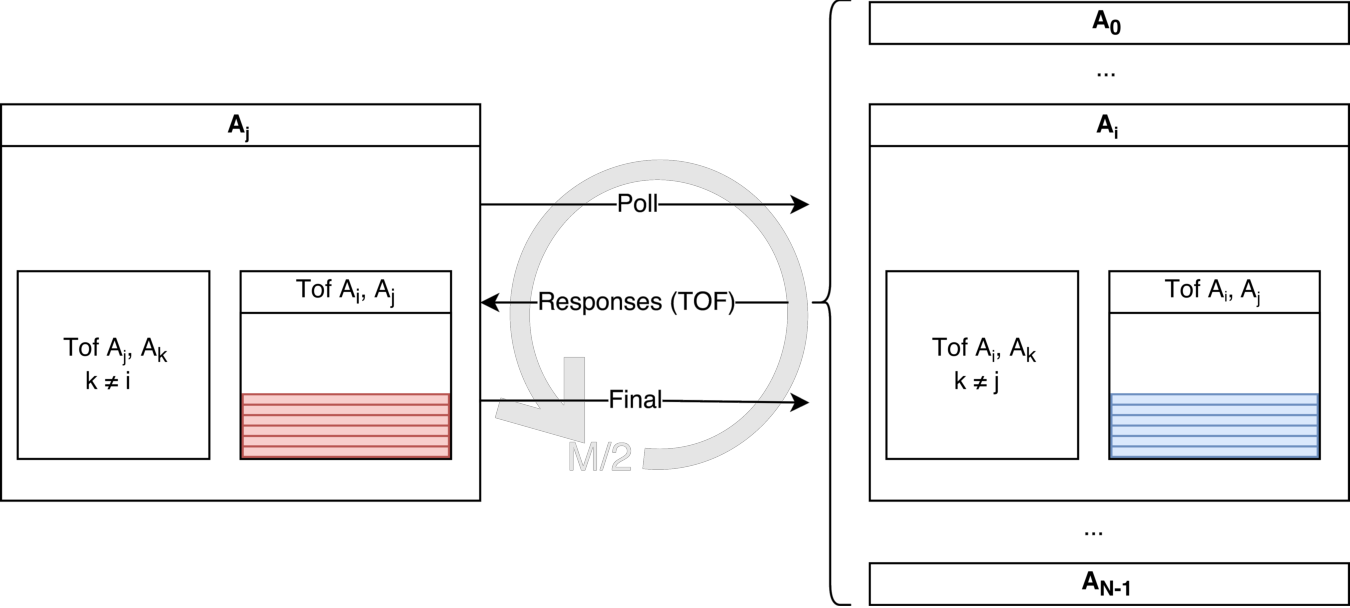
\includegraphics[width=\linewidth]{new_autoranging_3.pdf}
  \end{center}
\end{frame}

\begin{frame}{Simmetria - esempio}
  L'ancora $A_i$ colleziona ulteriori $M/2$ misure
  \begin{center}
    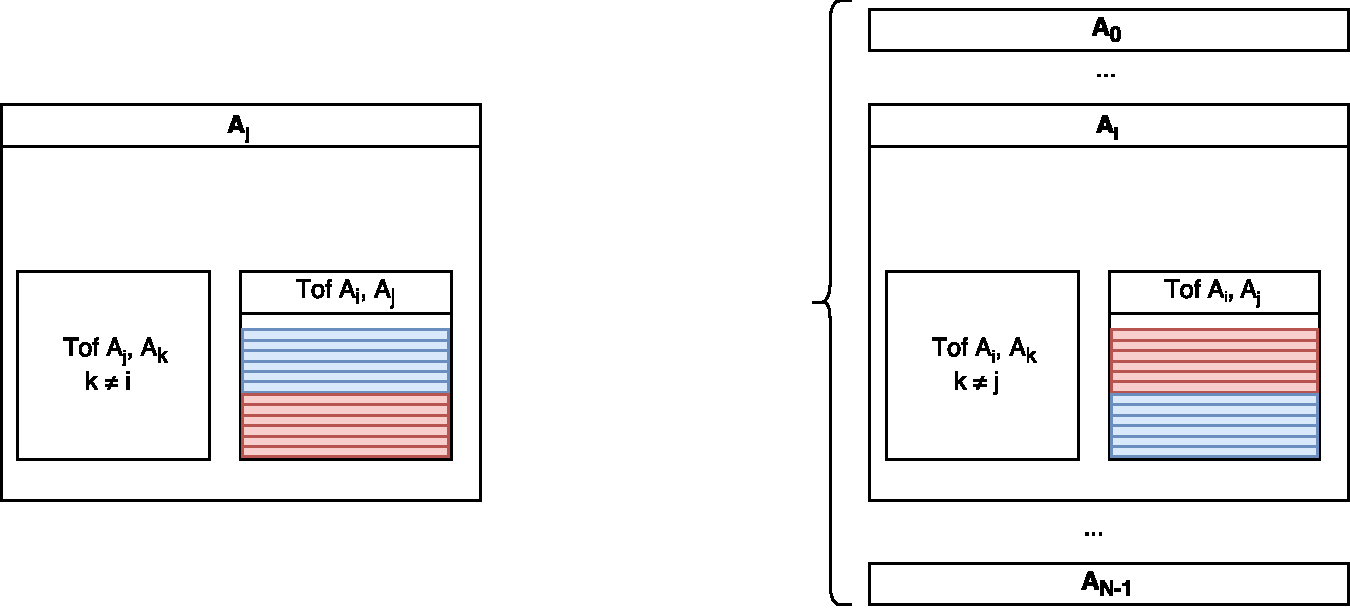
\includegraphics[width=\linewidth]{new_autoranging_4.pdf}
  \end{center}
\end{frame}

\begin{frame}{Simmetria - esempio}
  Le distribuzioni delle misure raccolte sfruttando la simmetria sono simili 
  \begin{center}
    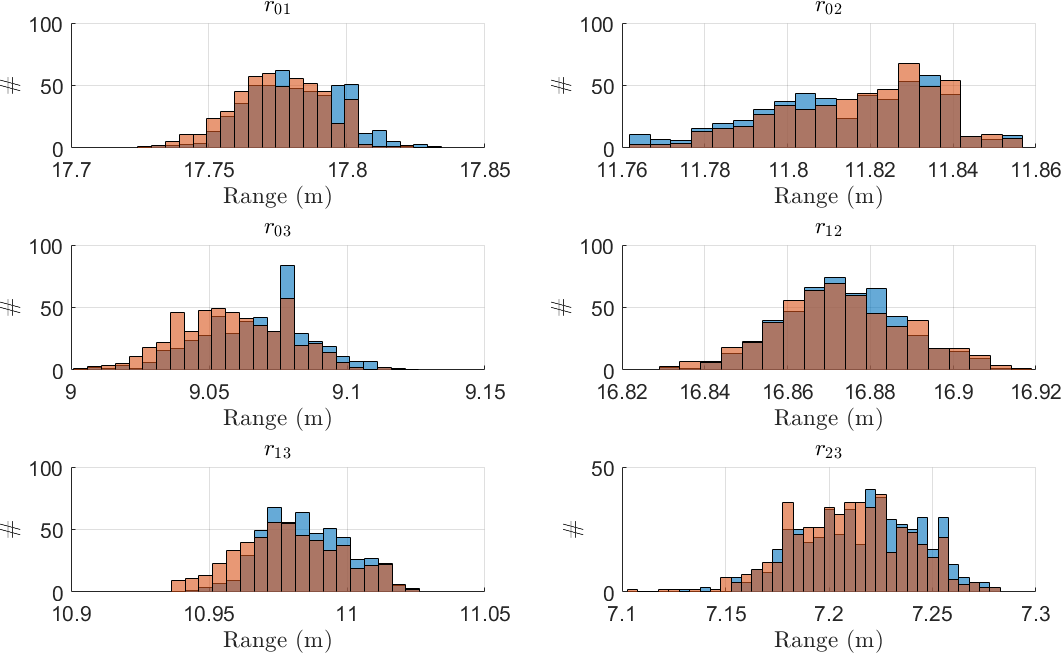
\includegraphics[scale=0.37]{autoranging.png}
  \end{center}
\end{frame}
